\documentclass[12pt, letterpaper]{article}
\usepackage[utf8]{inputenc}
\usepackage{amsmath}
\usepackage{changepage}% http://ctan.org/pkg/changepage
\usepackage{titlesec} 
\usepackage{commath}
\usepackage{placeins}
\usepackage{caption}
\usepackage{setspace}
\usepackage{subfig}
\usepackage{graphicx}
\usepackage{authblk}
\newcommand\tab[1][1cm]{\hspace*{#1}}
\titleformat{\subsection}[runin]{}{}{}{}[]
\onehalfspacing


\title{CS 260B Homework 1}
\author{Hanna Co}
\affil{Collaborators: Isha Gonugunta}
\date{Due: April 13, 2022}

\begin{document}
\maketitle
\newpage
\noindent \large{\textbf{(1a)} } \\
$f(x,y) = x^2-y^2$ and $x_0 = (0,0)$\\
We can compute the gradient of $f$: $\nabla f(x,y)=\langle 2x,-2y \rangle$\\
At $x_0$, the gradient is zero: $\nabla f(0,0)=\langle 0,0 \rangle$\\
However, $x_0$ is neither a local minimum or local maximum, and we can prove this through the second partial derivative test. We compute $H=f_{xx}(x,y)*f_{yy}(x,y)-f_{xy}(x,y)^2$. If $H>0$ then $(x,y)$ is either a local maximum or minimum; if $H<0$, then $(x,y)$ is a saddle point. We compute the second order partial derivatives:\\
$f_{xx}=2$\\
$f_{yy}=-2$\\
$f_{xy}=0$\\
$H=(2)(-2)+0^2=-4$, and $-4<0$, so $x_0$ is not a local maximum or minimum. Thus, for the function $f(x,y) = x^2-y^2$ and point $x_0 = (0,0)$, the gradient at $x_0$ is 0, but $x_0$ is not necessarily a local max or min, therefore the condition that $\nabla f(x,y)=0$ is necessary but not sufficient for a point to be a local max or min.

\newpage
\noindent \large{\textbf{(1b)} } \\
The gradient descent algorithm gives us $w_{i+1}=w_i+t\nabla f(w_i)$\\
Thus, $\lVert w_{i+1}-w_1\rVert$ is equivalent to $\lVert w_i+t\nabla f(w_i)-w_i\rVert$\\
$\lVert w_{i+1}-w_1\rVert = t\lVert \nabla f(w_i)\rVert$\\
This means that, each iteration, the decrease is proportional to the magnitude of the gradient. As we also know, the further away we are from a minimum or maximum, the larger the gradient is at that point.We are able to deduce this from the monotonicity of gradient descent.Thus, the closer we get to a minimum or maximum, the smaller steps we take. Therefore, with each GD iteration, we take smaller and smaller steps, until we reach a point where $\lVert \nabla f(w)\rVert \leq \epsilon$. \\
\\
From monotonicity, we know that $f(x_{i+1})\leq f(x_i)-\frac{t}{2}\lVert \nabla f(x_i)\rVert^2$.\\
As we run iterations of GD, we get\\
$f(w_1)\leq f(w_0)-\frac{t}{2}\lVert \nabla f(w_0)\rVert^2$\\
$f(w_2)\leq f(w_1)-\frac{t}{2}\lVert \nabla f(w_1)\rVert^2$\\
$f(w_3)\leq f(w_2)-\frac{t}{2}\lVert \nabla f(w_2)\rVert^2$\\
and so on.\\
We add up these inequalitites to get\\
$f(w_1)+f(w_2)+f(w_3)\leq f(w_0)-\frac{t}{2}\lVert \nabla f(w_0)\rVert^2+f(w_1)-\frac{t}{2}\lVert \nabla f(w_1)\rVert^2+f(w_2)-\frac{t}{2}\lVert \nabla f(w_2)\rVert^2$\\
$f(w_3)\leq f(w_0)-\frac{t}{2}(\lVert \nabla f(w_0)\rVert^2+\lVert \nabla f(w_1)\rVert^2+\lVert \nabla f(w_2)\rVert^2)$\\
We generalize this for $i$ iterations.\\
$f(w_i)\leq f(w_0)-\frac{t}{2}(\sum_{n=0}^{i=i-1} (\lVert \nabla f(w_n)\rVert^2)$\\
$f(w_i)-f(w_0)\leq -\frac{t}{2}(\sum_{n=0}^{i=i-1} (\lVert \nabla f(w_n)\rVert^2)$\\
$\sum_{n=0}^{i=i-1} \lVert \nabla f(w_n)\rVert^2\leq \frac{2}{t}(f(w_0)-f(w_i))$\\
The minimum value that $\lVert \nabla f(w_n)\rVert$ can take on is $\epsilon$, so\\
$i*\epsilon^2\leq \frac{2}{t}(f(w_0)-f(w_i))$\\
Thus\\
$i\leq \frac{2(f(w_0)-f(w_i))}{t*\epsilon^2}$\\
We want $i$ such that $f(w_i)$ is essentially the minimum, so\\
$i\leq \frac{2(f(w_0)-f(w))}{t*\epsilon^2}$\\
Thus, GD would take $\frac{2(f(w_0)-f(w))}{t*\epsilon^2}$ iterations to find such a $w$.

\newpage
\noindent \large{\textbf{(2)} } \\
From lecture, we know that for a $\beta$-smooth and convex function, \\
$f(x_{k+1})-f(x^*)\leq \frac{\beta}{2}(\lVert x_k-x^*\rVert^2-\lVert x_{k+1}-x^*\rVert^2)$\\
$f(x_k)-f(x^*)\leq \frac{\beta}{2}(\lVert x_{k-1}-x^*\rVert^2-\lVert x_k-x^*\rVert^2)$\\
\\
We are given\\
$f(y)\geq f(x)+\langle \nabla f(x),y-x\rangle + \frac{\alpha}{2}\lVert y-x\rVert^2_2$\\
Substituting in $y=x_k$ and $x=x^*$:\\
$f(x_k)\geq f(x^*)+\langle \nabla f(x^*),x_k-x^*\rangle + \frac{\alpha}{2}\lVert x_k-x^*\rVert^2_2$\\
$f(x_k)-f(x^*)\geq \frac{\alpha}{2}\lVert x_k-x^*\rVert^2_2$\\
$\frac{\alpha}{2}\lVert x_k-x^*\rVert^2_2\leq f(x_k)-f(x^*)$\\
We substitute in the equation from lecture:\\
$\frac{\alpha}{2}\lVert x_k-x^*\rVert^2_2\leq \frac{\beta}{2}(\lVert x_{k-1}-x^*\rVert^2-\lVert x_k-x^*\rVert^2)$\\
$\frac{\alpha}{\beta}\lVert x_k-x^*\rVert^2_2\leq \lVert x_{k-1}-x^*\rVert^2-\lVert x_k-x^*\rVert^2$\\
$\frac{\alpha}{\beta}\lVert x_k-x^*\rVert^2_2+\lVert x_k-x^*\rVert^2\leq \lVert x_{k-1}-x^*\rVert^2$\\
$(1+\frac{\alpha}{\beta})\lVert x_k-x^*\rVert^2_2\leq \lVert x_{k-1}-x^*\rVert^2$\\
$\lVert x_k-x^*\rVert^2_2\leq (1+\frac{\alpha}{\beta})^{-1}\lVert x_{k-1}-x^*\rVert^2$\\
As we iterate GD:\\
$\lVert x_k-x^*\rVert^2_2\leq (1+\frac{\alpha}{\beta})^{-1}\lVert x_{k-1}-x^*\rVert^2$\\
$\lVert x_k-x^*\rVert^2_2\leq (1+\frac{\alpha}{\beta})^{-1}(1+\frac{\alpha}{\beta})^{-1}\lVert x_{k-2}-x^*\rVert^2$\\
...\\
$\lVert x_k-x^*\rVert^2_2\leq \lVert x_0-x^*\rVert^2\prod_{i=0}^{k-1}(1+\frac{\alpha}{\beta})^{-1}$\\
Giving us\\
$\lVert x_k-x^*\rVert^2_2\leq (1+\frac{\alpha}{\beta})^{-k}\lVert x_0-x^*\rVert^2$\\
as desired.


\newpage
\noindent \large{\textbf{(3)} } \\
Suppose $f$ is convex, and $x^*$ is a local minimum in some interval $W$ of $f$. This means for all $x \in W$, $f(x)\geq f(x^*)$. Now say we have some point $y$ such that $f(y)<f(x^*)$. From convexity, we know that\\
 $f(\lambda x^*+(1-\lambda )y) \leq \lambda f(x^*)+(1-\lambda )f(y)$. \\
Since $f(y)<f(x^*)$ must be true, \\
$f(\lambda x^*+(1-\lambda )y) \leq \lambda f(x^*)+(1-\lambda )f(y) < f(\lambda x^*+(1-\lambda )x^*) \leq \lambda f(x^*)+(1-\lambda )f(x^*)$.\\
We simplify this expression to get the following:\\
$f(\lambda x^* +(1-\lambda )y) < f(x^*)$.\\
But, since $\lambda \in [0,1]$, and $x^*$ is a local minimum,  $f(\lambda x^*+(1-\lambda )y) > f(x^*)$ must hold. Therefore, we have a contradiction, so $x^*$ must also be a global minimum.

\newpage
\noindent \large{\textbf{(4a)} } \\
Taking the derivative for $\sigma(\langle w,x_i \rangle )$:\\
$\sigma(\langle w,x_i \rangle )=(1+e^{-\langle w,x_i\rangle})^{-1}$\\
$\sigma '(\langle w,x_i \rangle )=-(1+e^{-\langle w,x_i\rangle})^{-2}(-x_i e^{-\langle w,x_i\rangle})$\\
$\sigma '(\langle w,x_i \rangle )=\frac{x_{ik} e^{-\langle w,x_i\rangle}}{(1+e^{-\langle w,x_i\rangle})^{2}}$\\
$\sigma '(\langle w,x_i \rangle )=(x_{ik})(\sigma(\langle w,x_i \rangle )) * \frac{e^{-\langle w,x_i\rangle}}{1+e^{-\langle w,x_i\rangle}}$\\
$\sigma '(\langle w,x_i \rangle )=(x_{ik})(\sigma(\langle w,x_i \rangle ))(1-\sigma(\langle w,x_i \rangle ))$\\
\\
We can now find the gradient of $L(w)$:\\
$L(w)=(\frac{1}{n})\sum_{i=1}^{n}-y_i log(\sigma(\langle w,x_i \rangle )) - (1-y_i)log(1-\sigma(\langle w,x_i\rangle))$\\
$\nabla L(w)=(\frac{1}{n})\sum_{i=1}^{n}-y_i \frac{\sigma '(\langle w,x_i \rangle )}{\sigma(\langle w,x_i \rangle )} - (1-y_i)\frac{-\sigma '(\langle w,x_i \rangle )}{1-\sigma(\langle w,x_i \rangle )}$\\
$\nabla L(w)=(\frac{1}{n})\sum_{i=1}^{n}-y_ix_{ik}(1-\sigma(\langle w,x_i \rangle ) )+(1-y_i)(x_{ik}\sigma(\langle w,x_i \rangle ))$\\
$\nabla L(w)=(\frac{1}{n})\sum_{i=1}^{n}-y_ix_{ik}(1-\sigma(\langle w,x_i \rangle ) )+x_{ik}\sigma(\langle w,x_i \rangle ) +y_ix_{ik}\sigma(\langle w,x_i \rangle )$\\
$\nabla L(w)=(\frac{1}{n})\sum_{i=1}^{n}x_{ik}(-y_i+y_i\sigma(\langle w,x_i \rangle ) +\sigma(\langle w,x_i \rangle ) -y_i\sigma(\langle w,x_i \rangle ))$\\
$\nabla L(w)=(\frac{1}{n})\sum_{i=1}^{n}x_{ik}(\sigma(\langle w,x_i \rangle ) - y_i)$\\



\newpage
\noindent \large{\textbf{(4b)} } \\
The code below was used for running the gradient descent algorithms.\\
\begin{figure}[h!]
  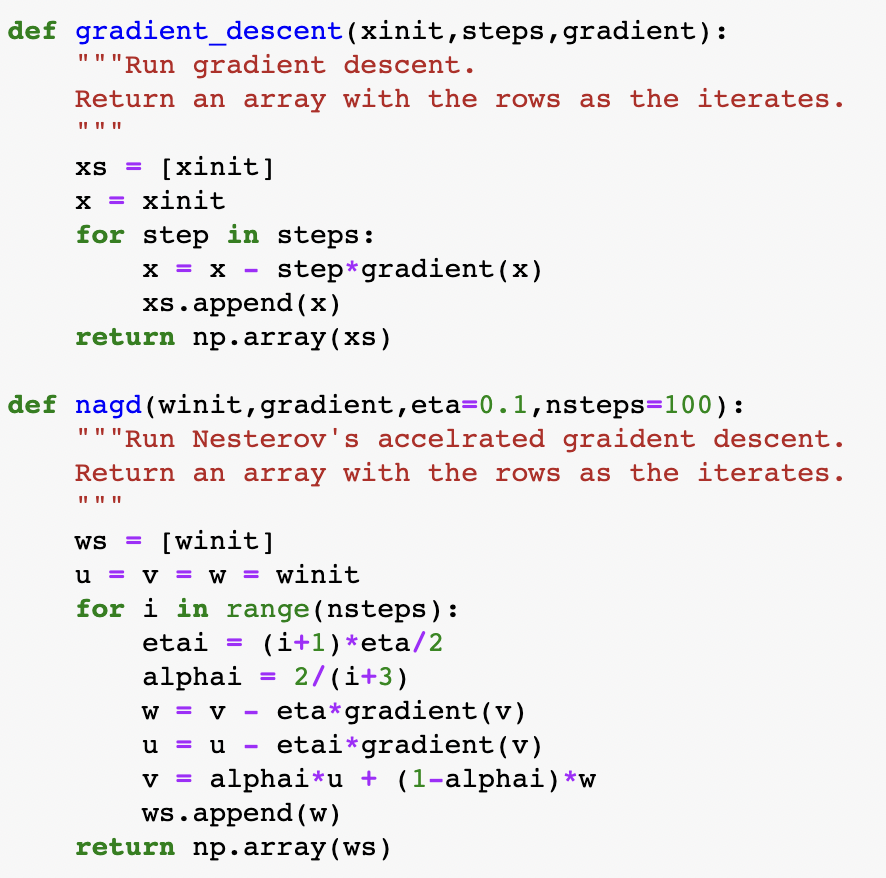
\includegraphics[scale=0.7]{./img/gd_nagd_code}
  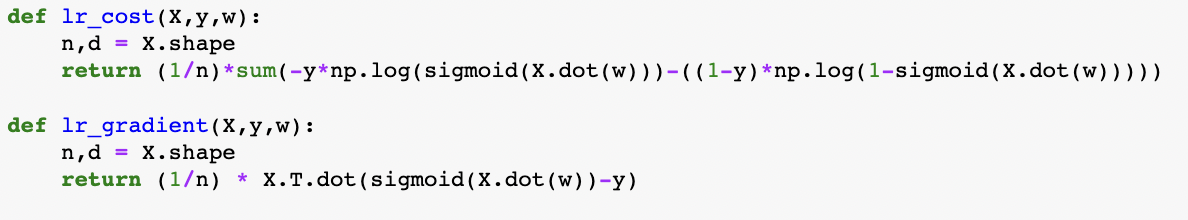
\includegraphics[scale=0.8]{./img/lr_funcs}
\end{figure}\\
\\
\begin{figure}[h!]
  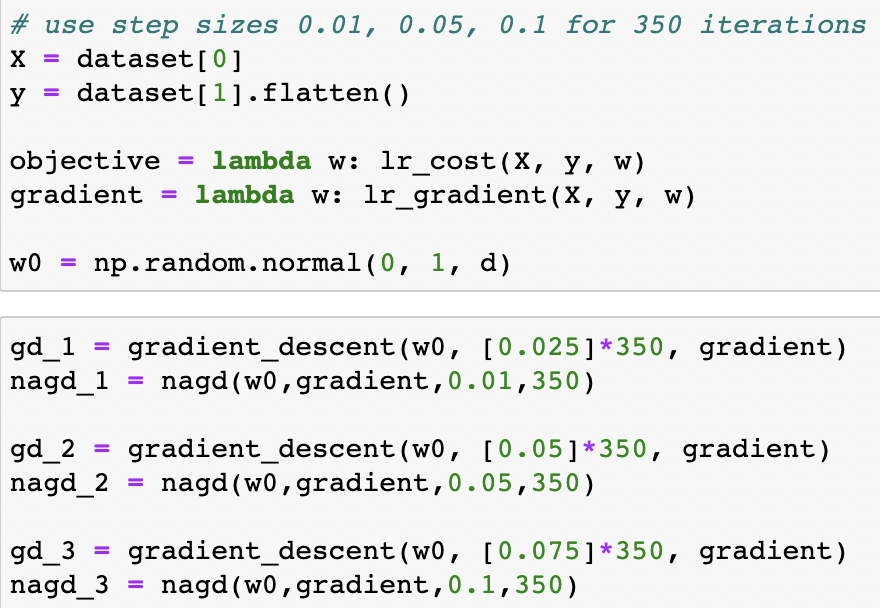
\includegraphics[scale=0.8]{./img/run_gd_code}
\end{figure}\\
\\
The following portion of code was used to generate plots for both GD and NAGD, with a separate plot for each step size. \\
\begin{figure}[h!]
  \centering
  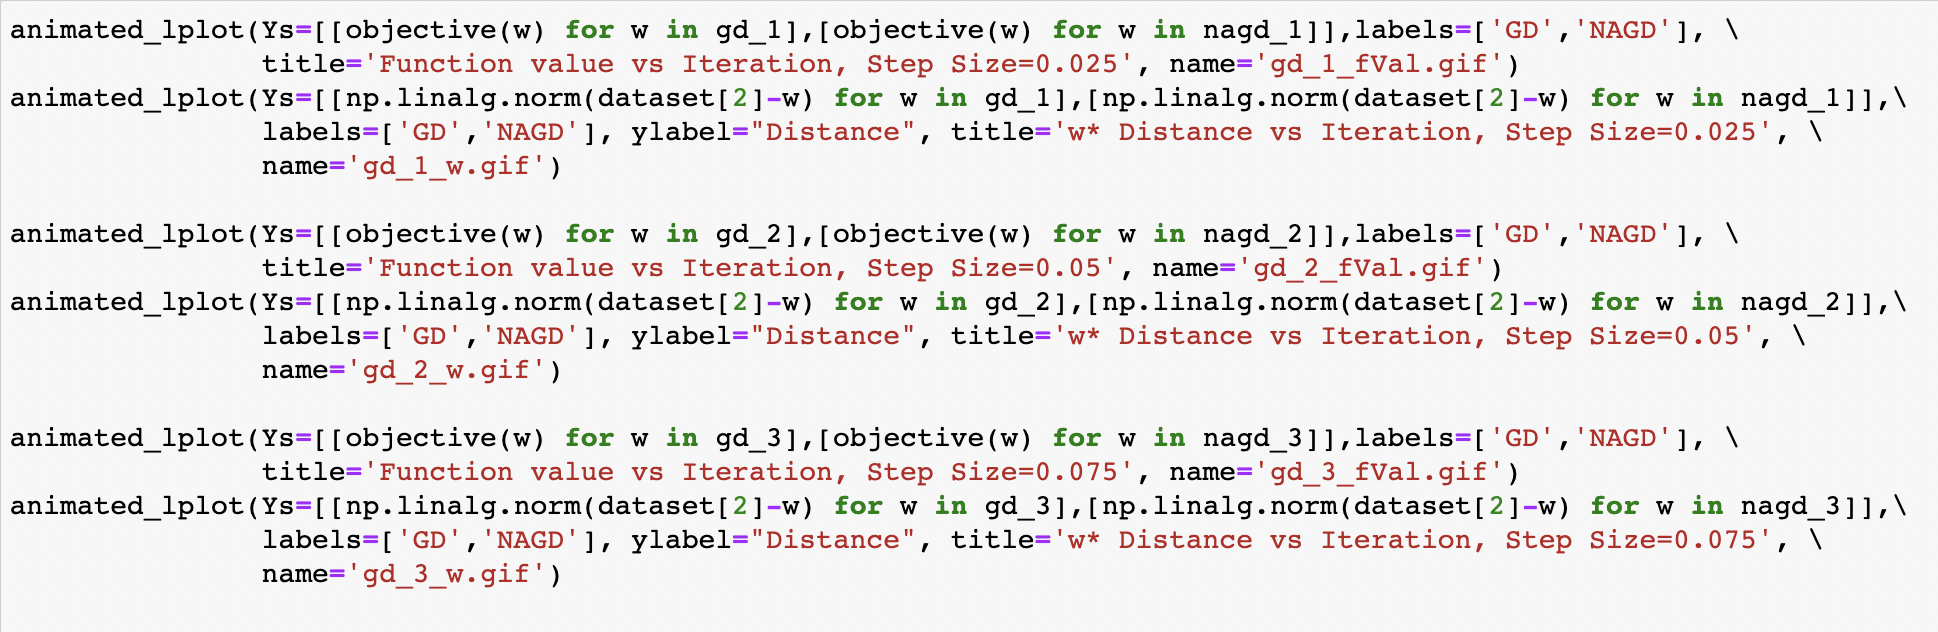
\includegraphics[scale=0.5]{./img/plots_by_step_size}
\end{figure}\\
\\
It produced the following plots.\\
\begin{figure}[h!]%
    \centering
    \subfloat[\centering Iteration vs f]{{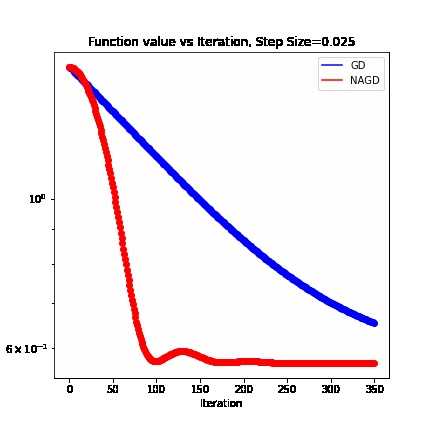
\includegraphics[width=6cm]{./img/gd_1_fVal} }}%
    \qquad
    \subfloat[\centering Distance from w*]{{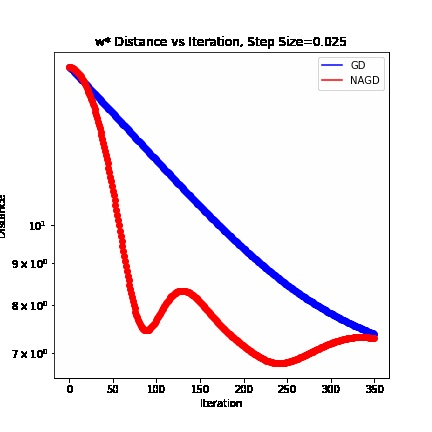
\includegraphics[width=6cm]{./img/gd_1_w} }}%
    \caption{Plots for Step Size 0.025}%
    \label{fig:example}%
\end{figure}
\begin{figure}[h!]%
    \centering
    \subfloat[\centering Iteration vs f]{{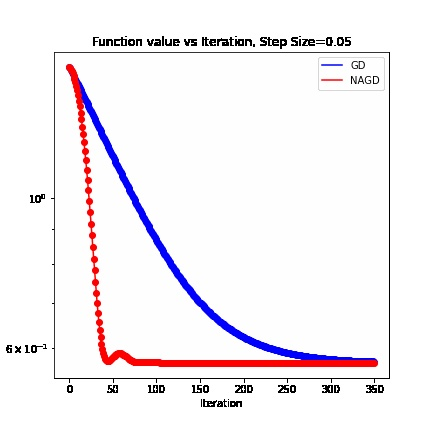
\includegraphics[width=6cm]{./img/gd_2_fVal} }}%
    \qquad
    \subfloat[\centering Distance from w*]{{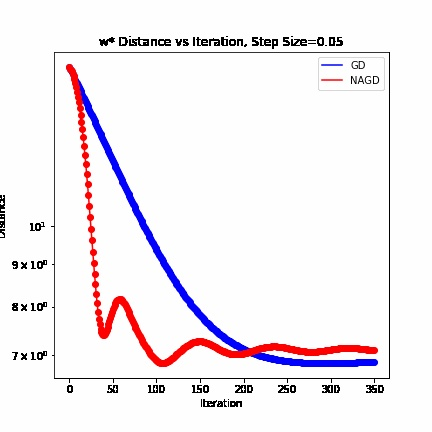
\includegraphics[width=6cm]{./img/gd_2_w} }}%
    \caption{Plots for Step Size 0.05}%
    \label{fig:example}%
\end{figure}
\begin{figure}[h!]%
    \centering
    \subfloat[\centering Iteration vs f]{{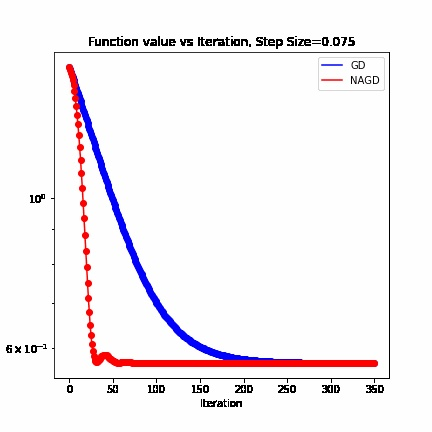
\includegraphics[width=6cm]{./img/gd_3_fVal} }}%
    \qquad
    \subfloat[\centering Distance from w*]{{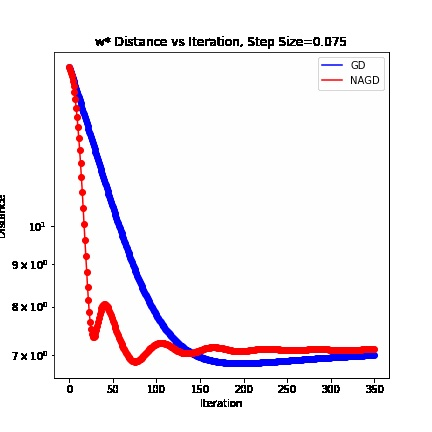
\includegraphics[width=6cm]{./img/gd_3_w} }}%
    \caption{Plots for Step Size 0.075}%
    \label{fig:example}%
\end{figure}\\
\\
For visualization purposes, I plotted all NAGD and GD iterations on the same plot with the following code.\\
\begin{figure}[h!]
  \centering
  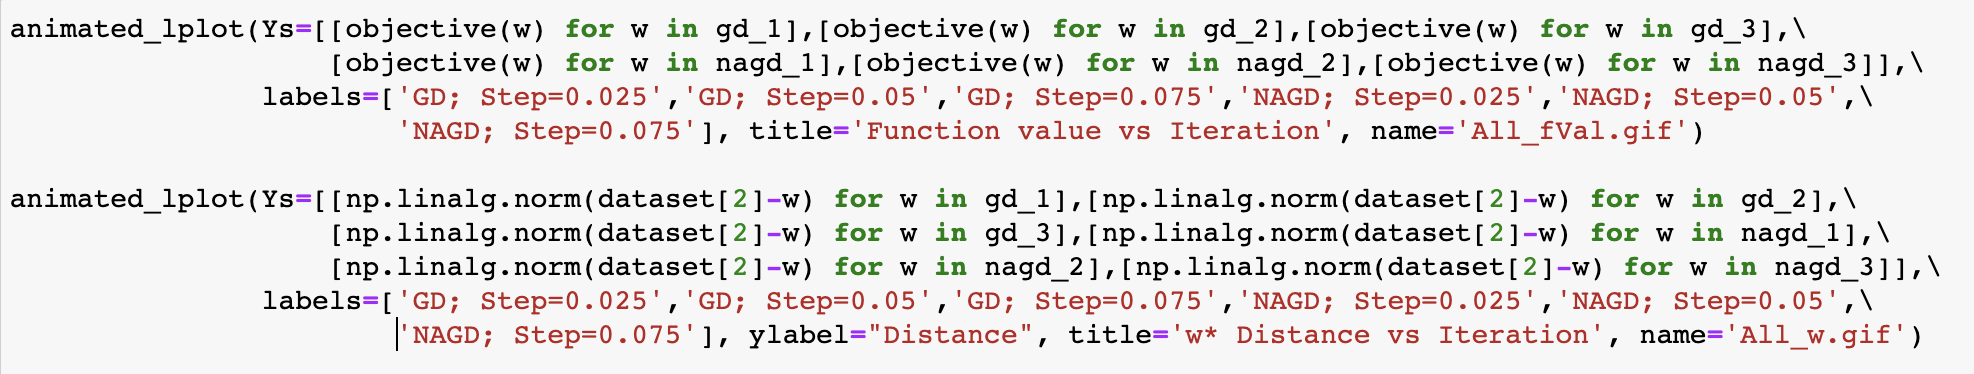
\includegraphics[scale=0.5]{./img/gd_nagd_plots}
\end{figure}\\
\\
This resulted in the following plots.\\
\begin{figure}[h!]%
    \centering
    \subfloat[\centering Iteration vs f]{{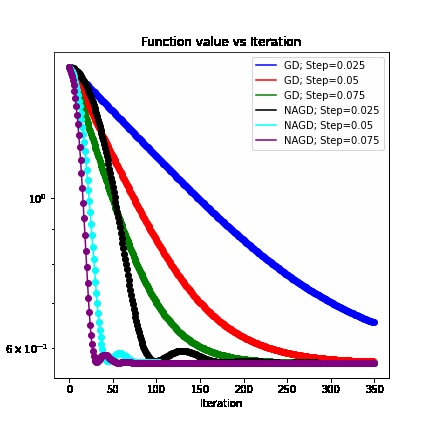
\includegraphics[width=6cm]{./img/All_fVal} }}%
    \qquad
    \subfloat[\centering Distance from w*]{{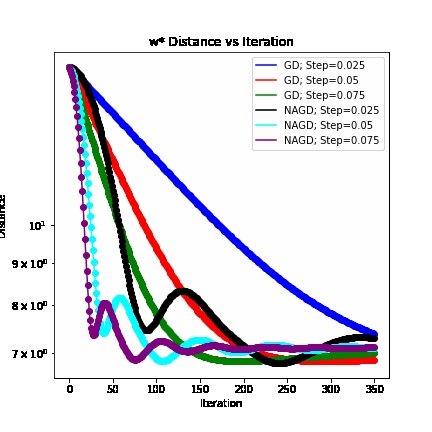
\includegraphics[width=6cm]{./img/All_w} }}%
    \caption{GD and NAGD for various step sizes}%
    \label{fig:example}%
\end{figure}\\
\\\\\\\\
This was very busy too look at, so I separated the GD and NAGD iterations into separate graphs.\\
\begin{figure}[h!]
  \centering
  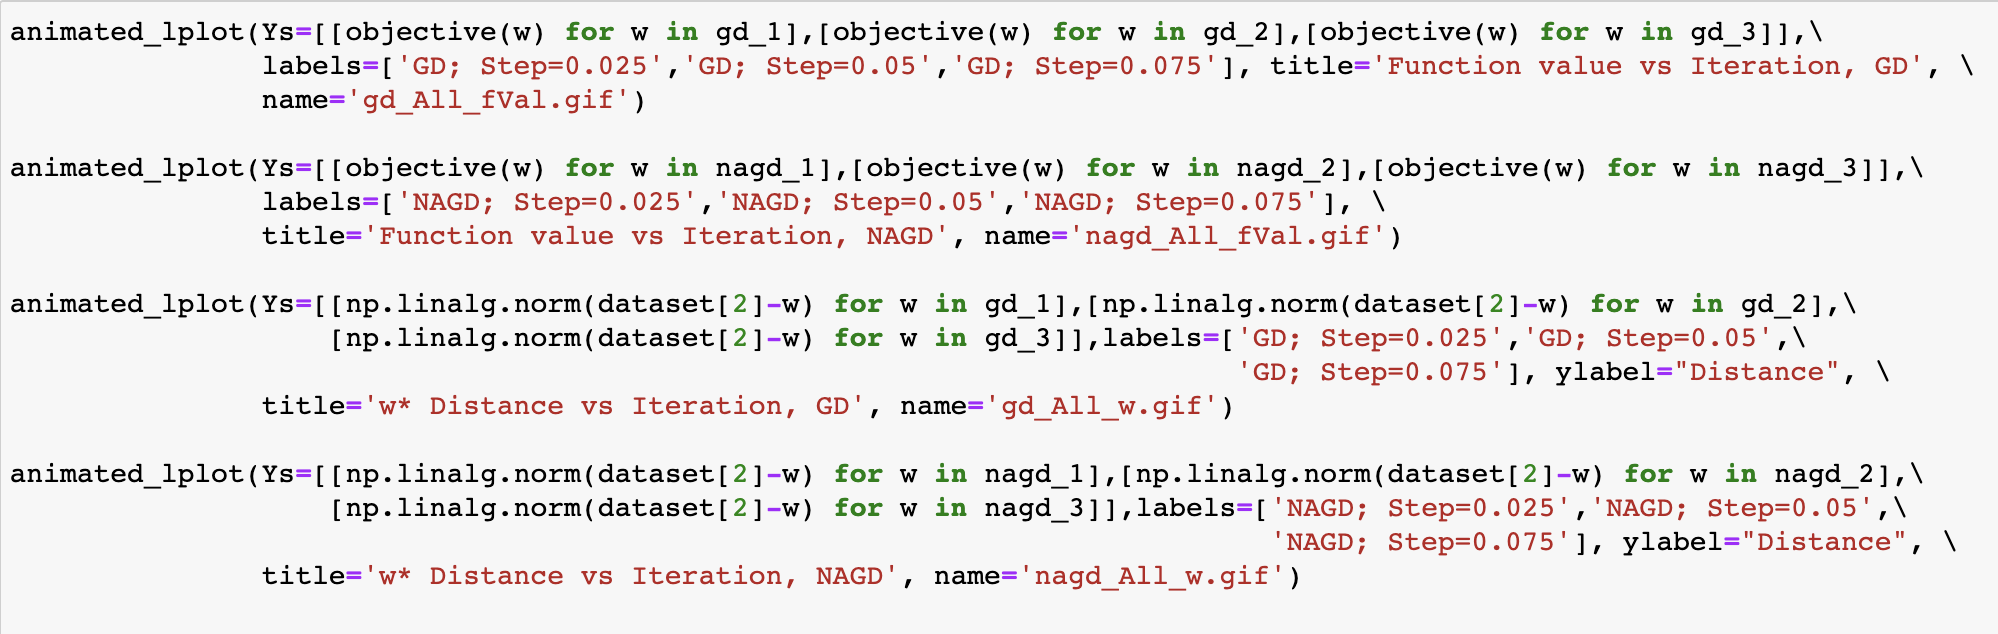
\includegraphics[scale=0.5]{./img/gd_nagd_separated_plots}
\end{figure}\\
\\
This resulted in the following plots.\\
\begin{figure}[h!]%
    \centering
    \subfloat[\centering Iteration vs f]{{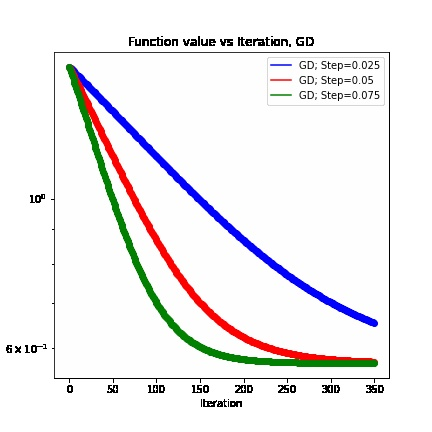
\includegraphics[width=6cm]{./img/gd_All_fVal} }}%
    \qquad
    \subfloat[\centering Distance from w*]{{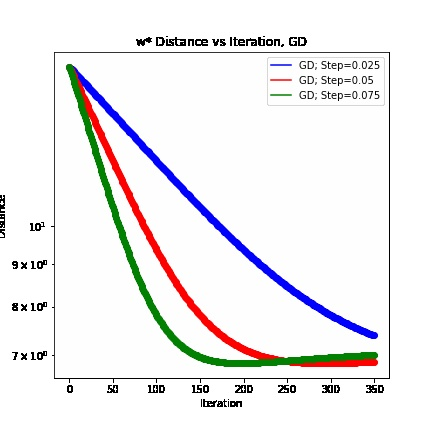
\includegraphics[width=6cm]{./img/gd_All_w} }}%
    \caption{GD Plots}%
    \label{fig:example}%
\end{figure}\\
\begin{figure}[h!]%
    \centering
    \subfloat[\centering Iteration vs f]{{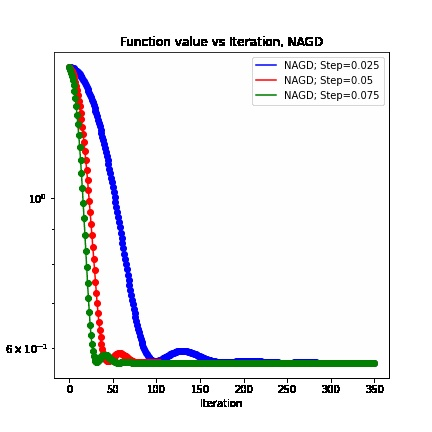
\includegraphics[width=6cm]{./img/nagd_All_fVal} }}%
    \qquad
    \subfloat[\centering Distance from w*]{{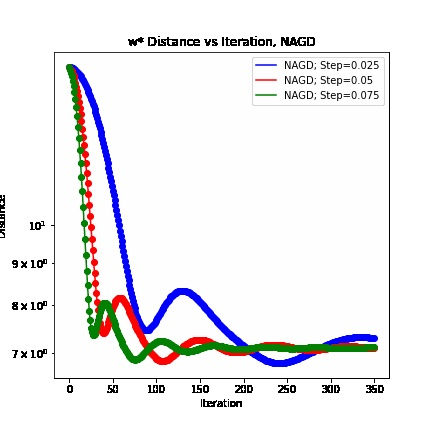
\includegraphics[width=6cm]{./img/nagd_All_w} }}%
    \caption{NAGD Plots}%
    \label{fig:example}%
\end{figure}\\

\end{document}